\documentclass[conference]{IEEEtran}
\hyphenation{op-tical net-works semi-conduc-tor}

\usepackage{epsfig,color}
%\def\Mcol{\sl\color{red}}
%\usepackage[french]{babel}
\usepackage{amssymb,amsfonts,amsmath,stmaryrd,amsthm}
\usepackage{url}
\usepackage{epstopdf}
\usepackage[noadjust]{cite}
\usepackage{array} 
\usepackage{tabularx}
\usepackage[ruled,vlined]{algorithm2e}
%\usepackage{amsmath}
\usepackage{dsfont}
%\usepackage{lipsum}
\usepackage{verbatim}
%\usepackage{algorithm}
\usepackage{gensymb}

\def\matlab{{\sc Matlab\ }}
\def\octave{{\sc Octave}}


\def\foorp{{\hfill$\spadesuit$}}
\def\ds{{\displaystyle}}
\def\inv{{^{-1}}}


% mathbb style

\def\AA{\mathbb A}
\def\BB{\mathbb B}
\def\CC{\mathbb C}
\def\DD{\mathbb D}
\def\EE{\mathbb E}
\def\FF{\mathbb F}
\def\GG{\mathbb G}
\def\HH{\mathbb H}
\def\II{\mathbb I}
\def\JJ{\mathbb J}
\def\KK{\mathbb K}
\def\LL{\mathbb L}
\def\MM{\mathbb M}
\def\NN{\mathbb N}
\def\OO{\mathbb O}
\def\PP{\mathbb P}
\def\QQ{\mathbb Q}
\def\RR{\mathbb R}
\def\SS{\mathbb S}
\def\TT{\mathbb T}
\def\UU{\mathbb U}
\def\VV{\mathbb V}
\def\WW{\mathbb W}
\def\XX{\mathbb X}
\def\YY{\mathbb Y}
\def\ZZ{\mathbb Z}




\def\var#1{{\hbox{Var}\left\{#1\right\}}}
\def\Id{\mathbb 1}


\def\o{\overline}
\def\la{\langle}
\def\ra{\rangle}

\def\ch{{\rm ch}}
\def\sh{{\rm sh}}



\DeclareMathAlphabet{\mathpzc}{OT1}{pzc}{m}{it}


\def\cA{\mathcal A}
\def\cB{\mathcal B}
\def\cC{\mathcal C}
\def\cD{\mathcal D}
\def\cE{\mathcal E}
\def\cF{\mathcal F}
\def\cG{\mathcal G}
\def\cH{\mathcal H}
\def\cI{\mathcal I}
\def\cJ{\mathcal J}
\def\cK{\mathcal K}
\def\cL{\mathcal L}
\def\cM{\mathcal M}
\def\cN{\mathcal N}
\def\cO{\mathcal O}
\def\cP{\mathcal P}
\def\cQ{\mathcal Q}
\def\cR{\mathcal R}
\def\cS{\mathcal S}
\def\cT{\mathcal T}
\def\cU{\mathcal U}
\def\cV{\mathcal V}
\def\cW{\mathcal W}
\def\cX{\mathcal X}
\def\cY{\mathcal Y}
\def\cZ{\mathcal Z}




\def\sgn{\hbox{sgn}}
\def\supp{\hbox{supp}}
\def\mod{{\mathrm {mod}}}

% bold
\def\bA{{\mathbf A}}
\def\bB{{\mathbf B}}
\def\bC{{\mathbf C}}
\def\bD{{\mathbf D}}
\def\bE{{\mathbf E}}
\def\bF{{\mathbf F}}
\def\bG{{\mathbf G}}
\def\bH{{\mathbf H}}
\def\bI{{\mathbf I}}
\def\bJ{{\mathbf J}}
\def\bK{{\mathbf K}}
\def\bL{{\mathbf L}}
\def\bM{{\mathbf M}}
\def\bN{{\mathbf N}}
\def\bO{{\mathbf O}}
\def\bP{{\mathbf P}}
\def\bQ{{\mathbf Q}}
\def\bR{{\mathbf R}}
\def\bS{{\mathbf S}}
\def\bT{{\mathbf T}}
\def\bU{{\mathbf U}}
\def\bV{{\mathbf V}}
\def\bW{{\mathbf W}}
\def\bX{{\mathbf X}}
\def\bY{{\mathbf Y}}
\def\bZ{{\mathbf Z}}

\def\ba{{\mathbf a}}
\def\bb{{\mathbf b}}
\def\bc{{\mathbf c}}
\def\bd{{\mathbf d}}
\def\be{{\mathbf e}}
\def\bbf{{\mathbf f}}
\def\bg{{\mathbf g}}
\def\bh{{\mathbf h}}
\def\bi{{\mathbf i}}
\def\bj{{\mathbf j}}
\def\bk{{\mathbf k}}
\def\bl{{\mathbf l}}
\def\bm{{\mathbf m}}
\def\bn{{\mathbf n}}
\def\bo{{\mathbf o}}
\def\bp{{\mathbf p}}
\def\bq{{\mathbf q}}
\def\br{{\mathbf r}}
\def\bs{{\mathbf s}}
\def\bt{{\mathbf t}}
\def\bu{{\mathbf u}}
\def\bv{{\mathbf v}}
\def\bw{{\mathbf w}}
\def\bx{{\mathbf x}}
\def\by{{\mathbf y}}
\def\bz{{\mathbf z}}




\def\balpha{\boldsymbol{\alpha}}
\def\bbeta{\boldsymbol{\beta}}
\def\bgamma{\boldsymbol{\gamma}}
\def\bGamma{\boldsymbol{\Gamma}}
\def\bdelta{\boldsymbol{\delta}}
\def\bDelta{\boldsymbol{\Delta}}
\def\bepsilon{\boldsymbol{\epsilon}}
\def\bvarepsilon{\boldsymbol{\varepsilon}}
\def\bzeta{\boldsymbol{\zeta}}
\def\beta{\boldsymbol{\eta}}
\def\bvartheta{\boldsymbol{\vartheta}}
\def\btheta{\boldsymbol{\theta}}
\def\bTheta{\boldsymbol{\Theta}}
\def\bkappa{\boldsymbol{\kappa}}
\def\blambda{\boldsymbol{\lambda}}
\def\bLambda{\boldsymbol{\Lambda}}
\def\bmu{\boldsymbol{\mu}}
\def\bnu{\boldsymbol{\nu}}
\def\bxi{\boldsymbol{\xi}}
\def\bpi{\boldsymbol{\pi}}
\def\bPi{\boldsymbol{\Pi}}
\def\brho{\boldsymbol{\rho}}
\def\bsigma{\boldsymbol{\sigma}}
\def\btau{\boldsymbol{\tau}}
\def\bphi{\boldsymbol{\varphi}}
\def\bPhi{\boldsymbol{\Phi}}
\def\bpsi{\boldsymbol{\psi}}
\def\bPsi{\boldsymbol{\Psi}}
\def\bomega{\boldsymbol{\omega}}
\def\bOmega{\boldsymbol{\Omega}}

\def\bzero{\boldsymbol{0}}

% overline
\def\ox{\overline{x}}
\def\oy{\overline{y}}
\def\oz{\overline{z}}

% tilde
\def\tb{{\tilde{a}}}
\def\tb{{\tilde{b}}}
\def\tc{{\tilde{c}}}
\def\td{{\tilde{d}}}
\def\te{{\tilde{e}}}
\def\tf{{\tilde{f}}}
\def\tg{{\tilde{g}}}
\def\th{{\tilde{h}}}
\def\ti{{\tilde{i}}}
\def\tj{{\tilde{j}}}
\def\tk{{\tilde{k}}}
\def\tl{{\tilde{l}}}
\def\tm{{\tilde{m}}}
\def\tn{{\tilde{n}}}
\def\to{{\tilde{o}}}
\def\tp{{\tilde{p}}}
\def\tq{{\tilde{q}}}
\def\tr{{\tilde{r}}}
\def\ts{{\tilde{s}}}
\def\ttt{{\tilde{t}}}
\def\tu{{\tilde{u}}}
\def\tv{{\tilde{v}}}
\def\tx{{\tilde{x}}}
\def\ty{{\tilde{y}}}
\def\tz{{\tilde{z}}}

\def\tgamma{{\tilde\gamma}}
\def\tGamma{{\tilde\Gamma}}
\def\tsigma{{\tilde\sigma}}
\def\tpi{{\tilde\pi}}
\def\tpsi{{\tilde\psi}}
\def\trho{{\tilde\rho}}
\def\tX{{\tilde{X}}}
\def\tY{{\tilde{Y}}}
\def\S{{\tilde{S}}}
\def\T{{\tilde{T}}}

% hat
\def\hb{{\hat b}}
\def\he{{\hat e}}
\def\hh{{\hat h}}
\def\hk{{\hat k}}
\def\hp{{\hat p}}
% \def\ht{{\hat t}}
\def\hu{{\hat u}}
\def\hv{{\hat v}}
\def\hw{{\hat w}}
\def\hx{{\hat x}}
\def\hy{{\hat y}}
\def\hz{{\hat z}}
\def\hLambda{{\hat \Lambda}}
\def\hDelta{{\hat \delta}}
\def\hlambda{{\hat \lambda}}
\def\hdelta{{\hat \delta}}
\def\halpha{{\hat \alpha}}
\def\hbeta{{\hat \beta}}
\def\htheta{{\hat \theta}}
\def\hsigma{{\hat \sigma}}


% vectors (underline)
\def\b{{\underline{b}}}
\def\e{{\underline{e}}}
\def\h{{\underline{h}}}
\def\k{{\underline{k}}}
\def\m{{\underline{m}}}
\def\t{{\underline{t}}}
\def\u{{\underline{u}}}
\def\v{{\underline{v}}}
\def\w{{\underline{w}}}
\def\x{{\underline{x}}}
\def\y{{\underline{y}}}
\def\z{{\underline{z}}}

\def\X{{\underline{X}}}
\def\Y{{\underline{Y}}}
\def\S{{\underline{S}}}
\def\T{{\underline{T}}}

\def\Om{{\underline{\Omega}}}
%
% Matrices
\def\A{{\underline{\underline{A}}}}
\def\RX{{\underline{\underline{R}}_X}}

%
% Algebraic quantities
\def\rg#1{{\hbox{rg}\left(#1\right)}}

\def\syn#1{{\tilde{#1}}}

\def\mk{\color{red}}
\def\ffc{\color{blue}}

\newcommand{\argmin}{\mathop{\mathrm{argmin}}}
\newcommand{\diag}[1]{\mbox{diag}\left(#1\right)}
\newcommand{\prox}{\mathrm{prox}}
\newcommand{\eqdef}{\stackrel{\mathrm{def}}{=}}

\theoremstyle{plain}
\newtheorem{thm}{Theorem}
\newtheorem{lem}[thm]{Lemma}
\newtheorem{Prop}[thm]{Proposition}
\newtheorem*{cor}{Corollary}
\newtheorem{mydef}{Definition}


\begin{document}


\title{Plug-and-play approach for blind image separation with application to document image restoration}

\author{\IEEEauthorblockN{Xhenis Coba, Fangchen Feng, Azeddine Begdadi}
	\IEEEauthorblockA{\textit{Laboratoire de Traitement et Transport de l'Information (L2TI)} \\
		\textit{Université Sorbonne Paris Nord}\\
		Villetaneuse, France \\
		xhenis.coba@univ-paris13.fr, fangchen.feng@univ-paris13.fr, azeddine.beghdadi@univ-paris13.fr}
}	

\maketitle

\begin{abstract}
We consider the blind image separation problem for document restoration. The existing methods rely on the general properties of source images such as independence, sparsity, non-negativity, and correlation. Instead of looking for other characteristics, we show in this paper that image-specified properties can be exploited through the plug-and-play approach for separation. In particular, we show that the BM3D and Non-local Means denoising methods, which exploit the nonlocal property, lead to better image separation in terms of the convergence rate. We then apply the proposed approaches to document the image restoration problems and show the advantages of the proposed approaches by numerical evaluations. 
\end{abstract}


\section{Introduction}
Old documents often suffer from the problem of the show-through and bleed-through effect. Show-through is a front-to-back interference, mainly due to the scanning process and the transparency of the paper, which
causes the text in the verso side of the document to appear also in the recto side (and vice versa)~\cite{sharma2001show}. Bleed-through is an intrinsic front-to-back physical deterioration due to ink seeping and produces an effect similar to that of show-through~\cite{boccuto2019blind}. Despite the complex physical model of the process which depends on the features of the paper, the transmittance parameters, the reflectance of the verso, and the spreading of light in the paper~\cite{tonazzini2015non,martinelli2012nonlinear,moghaddam2009low,almeida2008wavelet}, the following nonstationary linear model is well adapted to these effects locally~\cite{boccuto2019blind}:

\begin{equation}
\label{eq: linear mixing}
\bx[i] = A \bs[i],
\end{equation}
where $i$ is the index of the image pixels. $\bs$ is the concatenation of the source images in grayscale $\bs[i] = [s_r[i], s_v[i]]^T$ where $s_r[i]$ and $s_v[i]$ are the recto and verso sides (with a horizontal flip) of the source images respectively. $\bx[i] = [x_r[i], x_v[i]]^T$ with $x_r[i]$ and $x_v[i]$ being the observed recto and verso side images. $A\in\CC^{2 \times 2}$ is the mixing matrix. The target of the document restoration is to recover the source images $\bs[i]$ from the observed recto-verso mixtures $\bx[i]$ without knowing the mixing matrix $A$. This problem falls in the framework of Blind Source Separation (BSS)~\cite{comon2010handbook}.


ICA~\cite{hyvarinen2004independent} is a classical method for BSS. It assumes that the sources are independent and looks for a demixing matrix such that the separated components are as independent as possible~\cite{tonazzini2004independent}. Despite the good results in numerious domains, since ICA methods rely on the higher-order statistics for the separation, they can not work if more than one of the sources follows the Gaussian distribution~\cite{nordhausen2018independent}. Sparsity Component Analysis (SCA) is another well studied approach for BSS~\cite{souidene2007blind, zibulevsky2001blind,bobin2007sparsity}. This approach assumes that the sources are sparse in the spatial or a transformed domain. The separation problem is then formulated in an optimization framework and the estimation of the mixing matrix and the source images are performed simultaneously. One of the advantages of the SCA compared to the ICA is that it leads to better results if the mixtures are degraded with additive noise~\cite{bobin2007sparsity}. It's also important to notice that several works are dedicated to exploiting the links between the ICA and SCA methods~\cite{feng2018revisiting,bronstein2005sparse,boukouvalas2018sparsity}.

Besides the independent and sparsity properties of the source images, other criteria have also been investigated for separation such as Non-negative Matrix Factorization (NMF)~\cite{merrikh2010using} and Canonical Correlation Analysis (CCA)~\cite{boccuto2019blind} for the document restoration application. 

For blind image separation, in the determined scenario, the demixing matrix is estimated based on different characteristics of the source images. On the other hand, image denoising methods seek to remove perturbations or errors from the observed images based on the characteristics of images. Extensive research has been carried out on image denoising over the past three decades, which has led to highly optimized algorithms. In this paper, instead of searching for other characteristics for blind image separation, we propose to use the existing denoising approaches in a plug-and-play way for the separation. In particular, we show that the BM3D~\cite{dabov2007image} and the Nonlocal Mean~\cite{buades2005non} denoising methods lead to better separation than the existing approaches in terms of ??. It's the first time, to the best of our knowledge, that the BM3D and Nonlocal mean are used for image separation.

The contribution of the paper is as follows:

The reminder of this paper is organized as follows. In Section~\ref{sec: plug and play}, we describe the proposed separation approach with plug-and-play. We then apply the appraoch for the document restoration problem in Section~\ref{sec: document restoration}. The numerical evaluations are performed in Section~\ref{sec: xp} and we conclude the paper in Section~\ref{sec: conclusion}.  


\section{Plug-and-play approach for image separation}
\label{sec: plug and play}

\subsection{Optimization framework}
Both ICA and SCA in the determined case can be formulated into the optimization framework~\cite{feng2018revisiting} as follows:
\begin{equation}
\label{eq: optimization framework}
\argmin_{W, \bs} \frac{1}{2} \|W\bx - \bs\|_F^2 + \mathcal{P}(\bs) + \mathcal{G}(W),
\end{equation}
where $W$ is the demixing matrix. $\|\cdot\|_F$ denotes the Frobenius norm of matrix. $\mathcal{P}(\bs)$ is the penalty term based on the characterestics of the source images. $\mathcal{G}(W)$ is the constraint of the demixing matrix. For ICA approaches, $\mathcal{P}(\bs)$ is the independence measurement for the sources and $\mathcal{G}(W)$ is the unitary constaint which leads to the decorrelation constraint of the sources, along with the whitening pre-processing. For SCA, $\mathcal{P}(\bs)$ is the sparse penalty in the spatial or a transformed domain and $\mathcal{G}(W)$ is the unit-norm constraint of the estimated mixing matrix.

The above optimization problem~\eqref{eq: optimization framework} in the general form can be solved with the iterative alternating minimization~\cite{tseng2001convergence}. In each iteration, we solve the two following sub-problems in an alternating way until convergence.:
\begin{equation}
\label{eq: subpb1}
	\argmin_{\bs} \frac{1}{2} \|W\bx - \bs\|_F^2 + \mathcal{P}(\bs),
\end{equation}
and 
\begin{equation}
\label{eq: subpb2}
\argmin_{W} \frac{1}{2} \|W\bx - \bs\|_F^2 + \mathcal{G}(W).
\end{equation}

The sub-problem~\eqref{eq: subpb1} is directly related to the classical denoising problem for additive Gaussian noise. The plug-and-play~\cite{venkatakrishnan2013plug,chan2016plug,ono2017primal} approach consists of replacing the denoising formulation by existing denoising approaches. It's important to note that the denoising algorithms do not necessarily correspond to any penalty term in closed form. In this paper, we illustrate the separation results using the Wavelet-based~\cite{donoho1994ideal,chang2000adaptive}, Total-Variation (TV) minimization~\cite{chambolle2004algorithm}, BM3D~\cite{dabov2007image}, and Non-local mean~\cite{buades2005non} denoising approaches.

The sub-problem~\eqref{eq: subpb2} can be solved with the gradient descend approach with the whitening projection. The proposed algorithm is resumed as follows:




\subsection{Related methods}
The proposed framework englobes several existing separation approaches. When the wavelet-based denoiser is used, the proposed approach is closely related to the method proposed in~\cite{ichir2003wavelet} and~\cite{kutyniok2010image}. When the TV denoiser is used, the proposed approach is related to the sparsity-based method in~\cite{souidene2007blind}. The approach is closely related to the methods discussed in~\cite{zhao2014blind} if the dictionary-learning approach is used as the denoiser.

\subsection{Dictionary learning for visual chirality}
For document image restoration from scanned recto-verso pages of document, the two original document images are mixed with one of them horizontally flipped. Recently, it's shown in~\cite{lin2020visual} that text is a strong signal for high-level visual chirality which is a fundemantal property of images. However, classical denoising approaches (Wavelet-based, TV minimization, BM3D, and Non-local mean) do not exploit such property of images. In this paper, we propose to use the dictionary-learning~\cite{elad2006image} approach to exploit such property. More precisely, we...



\section{Numerical evaluation}
\label{sec: xp}
We first test the proposed approach in a general case for natural scene images. We then investigate the application of the proposed approach for document restoration in various scenarios.

\subsection{Plug and play in a general case}

 
 
\subsection{Separation for document image restoration}
 the mixing matrix should be symmetric or not~\cite{tonazzini2007fast}?

 \begin{figure}[ht!]
	\centering
	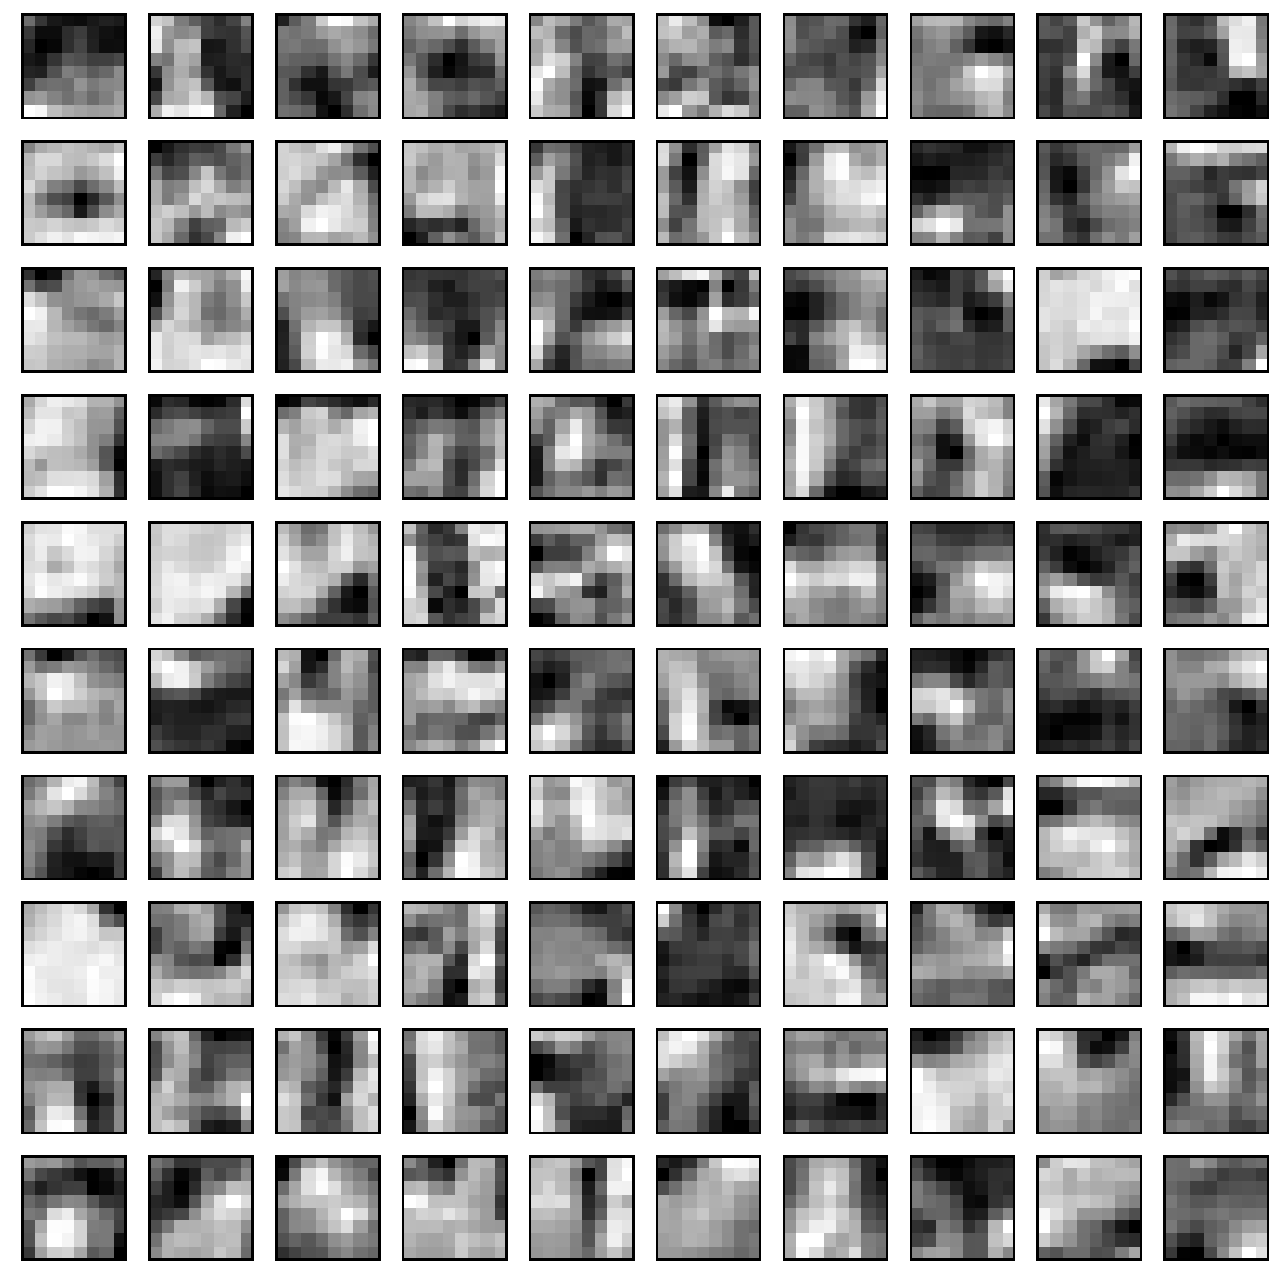
\includegraphics[width=0.5\linewidth]{./fig/dictionary.pdf}
	\caption{The learned dictionary.}
	\label{fig: dictionary result}
\end{figure}


 \begin{figure*}[ht!]
	\centering
	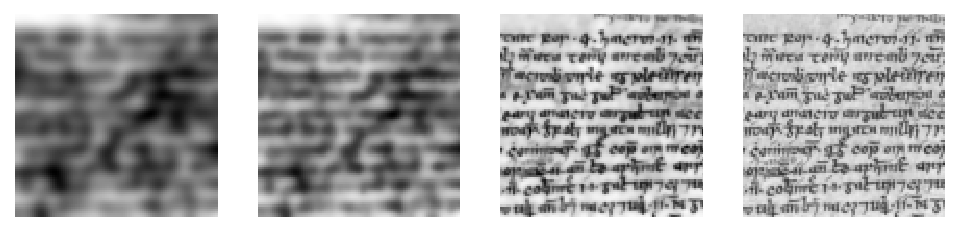
\includegraphics[width=\linewidth]{./fig/test.pdf}
	\caption{The denoising results of TV with different $\sigma$.}
	\label{fig: TV denoiser}
\end{figure*}

 \begin{figure*}[ht!]
	\centering
	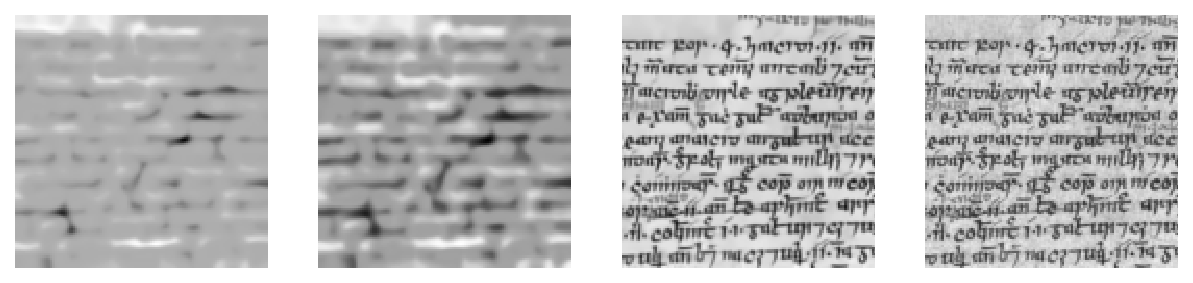
\includegraphics[width=\linewidth]{./fig/test_bm3d.pdf}
	\caption{The denoising results of BM3D with different $\sigma$.}
	\label{fig: bm3d denoiser}
\end{figure*}

\section{Conclusion}
\label{sec: conclusion}
For determined blind image separation problem, we show that the denoisers can be used for separation. Further denoiser can also be directly applied for separation task.


\bibliographystyle{IEEEbib}
\bibliography{biblio}

\end{document}
